\begin{ex}
 Duas máquinas A e B produzem peças idênticas, sendo que a produção da máquina A é o triplo da produção da máquina B. A máquina A produz 80\% das peças boas e a máquina B produz 90\%.Uma peça é selecionada ao acaso no estoque e verifica-se que é uma peça boa. Qual a probabilidade de que tenha sido fabricada pela máquina A?
 
   \begin{sol}
    Acompanhe o diagrama
    \\
    \\
     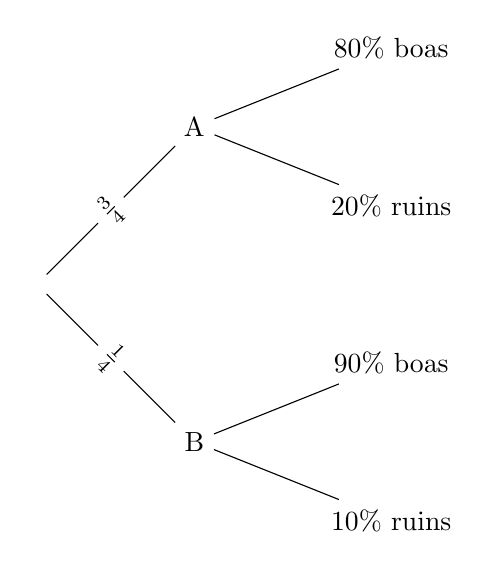
\begin{tikzpicture} [grow=right,sloped]
      \tikzstyle{level 1} = [sibling distance = 4.0 cm, level distance = 2.0 cm]
        \tikzstyle{level 2}=[sibling distance = 2.0 cm, level distance= 2.5 cm]
          \node{}
            child{
              node{B}
                 child{
                    node{10\% ruins}
                 }
                 child{
                    node{90\% boas}
                 }
            edge from parent
            node[fill=white]{\(\frac{1}{4}\)}
            }
          child{
             node{A}
                child{
                  node{20\% ruins}
                }
                child{
                  node{80\% boas }
                }
            edge from parent
            node[fill=white]{\(\frac{3}{4}\)}
            };
        \end{tikzpicture}
        \\
        $\frac{3}{4}\cdot80\%=\frac{3}{5}$
        
  \end{sol}
\end{ex}